\documentclass[conference]{IEEEtran}
\IEEEoverridecommandlockouts

\usepackage{cite}
\usepackage{amsmath,amssymb,amsfonts}
\usepackage{algorithmic}
\usepackage{graphicx}
\usepackage{textcomp}
\usepackage{xcolor}
\usepackage{booktabs}
\usepackage{microtype}
\usepackage{url}
\usepackage{hyperref}

\hypersetup{
    colorlinks=true,
    linkcolor=black,
    citecolor=black,
    urlcolor=black
}

\def\BibTeX{{\rm B\kern-.05em{\sc i\kern-.025em b}\kern-.08em
    T\kern-.1667em\lower.7ex\hbox{E}\kern-.125emX}}

\begin{document}

\title{Cross-Session Fingerprint Consistency for Adaptive Bot Detection in QUIC and Post-Quantum TLS}

\author{\IEEEauthorblockN{Anonymous Authors}
\IEEEauthorblockA{\textit{Department of Computer Science and Engineering} \\
\textit{Research Testbed on Transport Security and Automation}\\
\textit{Artifact Available at Repository}\\}
}

\maketitle

\begin{abstract}
The rollout of QUIC (HTTP/3) and hybrid post-quantum key encapsulation (e.g., X25519MLKEM768) has widened the TLS ClientHello into a significantly richer fingerprinting surface than the legacy space JA3 and JA4 methods were designed around. Whether this extra cryptographic and transport surface actually aids in distinguishing automated clients from genuine human users has not previously been measured under controlled adversarial conditions. In this work, we present a controlled, fully instrumented testbed of 1,820 live browsing sessions, organized into 455 repeat-visit identity groups against an HTTP/3 and post-quantum TLS-enabled origin. The testbed spans a five-tier adversary ladder ranging from naive HTTP script clients to an adaptive bot that negotiates HTTP/3, synthesizes post-quantum key shares, and normalizes inter-request pacing. On this corpus, we evaluate two consistency metrics layered atop raw protocol features: a spatial score measuring the information-theoretic surprise of single-session protocol combinations against an empirical human baseline, and a temporal score measuring fingerprint disagreement across sequential sessions belonging to a claimed identity.

Our findings establish four key results. First, against non-adaptive bots, post-quantum and QUIC protocol features provide zero measurable in-distribution gain over classical TLS features combined with behavioural pacing (both reaching an identical 0.9958 accuracy and 1.3\% human false-positive rate). Second, this in-distribution success is brittle: under a held-out adaptive adversary, all conventional models suffer catastrophic evasion of 95.9\% to 97.3\%. Third, cross-session temporal consistency restores detection, slashing evasion from 58.1\% to 18.9\% under default XGBoost ($p = 2 \times 10^{-6}$, McNemar test), and further to \textbf{14.9\%} with tuned hyperparameters and minority class weighting (stable across five random seeds at $16.5\% \pm 4.8\%$). On threshold-independent metrics, temporal consistency elevates human-vs.-adaptive-bot ROC-AUC from 0.795 to \textbf{0.943} and PR-AUC from 0.610 to \textbf{0.905}. Fourth, spatial consistency yields a mean absolute SHAP attribution of exactly zero due to feature collinearity and distribution collapse. We formalize a parametric closed-form risk formula ($C(s)$) and a group-level Noisy-OR aggregation rule that detects 81.0\% of adaptive groups. We conclude that cross-session temporal stability, rather than ephemeral per-handshake protocol detail, represents the sustainable signal against adversaries who understand modern fingerprinting schemas.
\end{abstract}

\begin{IEEEkeywords}
bot detection, adversarial machine learning, HTTP/3, QUIC, post-quantum cryptography, TLS fingerprinting, web security, traffic classification.
\end{IEEEkeywords}

\section{Introduction}
Automated web agents, crawlers, and credential-stuffing bots impose severe operational costs on modern web infrastructure \cite{hou2020botmeter}. For two decades, network-layer bot defenses have relied heavily on passive Transport Layer Security (TLS) fingerprinting. Because the cipher suite preference list, extension ordering, supported elliptic curves, and point formats are dictated by the underlying TLS client library rather than the end-user application code, hashing these parameters provides a robust fingerprint without decrypting traffic payload. Frameworks such as JA3 \cite{althouse2017ja3} and JA4 \cite{foxio2024ja4} formalized this paradigm and achieved widespread deployment across commercial Web Application Firewalls (WAFs) and Security Operations Centers (SOCs) \cite{anderson2016identifying}.

However, static handshake fingerprinting suffers from an inherent structural vulnerability: once a fingerprint is defined as a deterministic digest of client configuration, an adversary can mimic that configuration byte-for-byte \cite{vastel2020fp}. Advanced evasion frameworks (such as \texttt{curl-cffi} and anti-detect browser engines \cite{jordan2022synthetic}) intercept and synthesize arbitrary ClientHello messages, rendering static signature matching fragile \cite{biggio2013evasion}.

Two major protocol evolutions currently reshape web transport. First, QUIC \cite{rfc9000} integrates transport parameter negotiation directly into the cryptographic handshake, exposing transport version, connection identifier lengths, and active parameter counts at connection setup \cite{yu2021first, piraux2021observing}. Second, major web browsers have deployed hybrid post-quantum key exchange mechanisms (specifically X25519MLKEM768 \cite{fips203, rfc8446}) to protect traffic against retroactive decryption (``harvest now, decrypt later'') \cite{paquin2020benchmarking, cloudflare2024pq}. Because mainstream browsers now emit post-quantum key shares and negotiate HTTP/3 over UDP, whereas mainstream Python scraping tools and commodity proxies predominantly lag behind on standard TLS~1.3 over TCP, it is tempting to view these newly visible protocol fields as an intrinsic defensive advantage.

In this work, we rigorously test that assumption through empirical measurement. Our findings reveal that the premise is largely illusory: on conventional bots, post-quantum and QUIC protocol fields contribute nothing measurable beyond classical handshake features and basic request timing. Furthermore, when facing an adaptive adversary that deliberately synthesizes post-quantum key shares and negotiates QUIC, in-distribution models collapse completely, exhibiting up to 97.3\% evasion. 

What survives adversarial adaptation is an entirely different defensive primitive: \textbf{cross-session fingerprint consistency}. Genuine human clients maintain a highly consistent cryptographic stack across consecutive sessions from the same device or profile. Conversely, distributed bot operations—which frequently rotate across disparate residential proxy exit nodes, cloud worker instances, and protocol fallbacks—exhibit subtle cross-session drift.

This study is structured around three research questions:
\begin{itemize}
    \item \textbf{RQ1:} Do post-quantum key share and QUIC transport features improve detection of conventional bots beyond classical TLS fingerprinting and behavioural timing?
    \item \textbf{RQ2:} Which specific feature groups drive the observed in-distribution performance, and what role do protocol-level fields play?
    \item \textbf{RQ3:} How effectively do detection models withstand an adaptive adversary built with complete knowledge of the feature schema, and what signals remain viable?
\end{itemize}

\noindent\textbf{Contributions.} The primary contributions of this work are:
\begin{enumerate}
    \item \textbf{Instrumented Multi-Tier Testbed:} We construct an end-to-end testbed generating 1,820 live sessions across 455 repeat-visit identity groups, evaluated against an HTTP/3 and post-quantum TLS origin. The dataset encompasses a five-tier adversary ladder ranging from naive HTTP libraries to an adaptive bot combining post-quantum key share emulation, QUIC transport, and humanized request pacing.
    \item \textbf{Empirical Negative Result for Protocol Features:} We provide rigorous evidence that post-quantum and QUIC protocol presence signals offer no discriminative gain ($0.8000 \to 0.8000$ accuracy) over classical TLS features on conventional traffic, as behavioural timing dominates in-distribution classification (0.9958 accuracy).
    \item \textbf{Demonstration of Adversarial Fragility:} We show that models achieving near-perfect in-distribution accuracy invert completely under an adaptive adversary, suffering 95.9\% to 97.3\% evasion. In-distribution validation on saturated benchmarks is an active anti-indicator of operational security.
    \item \textbf{Temporal Consistency Defense:} We introduce a temporal inconsistency metric ($s_{\text{temporal}}$) that slashes adaptive evasion from 58.1\% to 18.9\% ($p = 2 \times 10^{-6}$, McNemar test) and further to \textbf{14.9\%} with tuned hyperparameters and minority class weighting. Multi-seed validation across five seeds yields $16.5\% \pm 4.8\%$. On threshold-independent metrics, temporal consistency boosts human-versus-adaptive-bot ROC-AUC from 0.795 to \textbf{0.943} and PR-AUC from 0.610 to \textbf{0.905}.
    \item \textbf{Parametric Risk Formulation and Deployment Analysis:} We distill the consistency signal into a closed-form logistic formula ($C(s)$) and a group-level Noisy-OR aggregation rule that detects 81.0\% of adaptive campaigns, and demonstrate its sub-millisecond suitability for line-rate WAF deployment.
\end{enumerate}

\section{Related Work}

\subsection{TLS Fingerprinting}
Passive fingerprinting of TLS clients originated with heuristics analyzing cipher suite preference lists and extension sets \cite{anderson2016identifying}. JA3 \cite{althouse2017ja3} standardized this into an MD5 digest of five ClientHello parameters: TLS version, accepted ciphers, extension list, supported elliptic curves, and elliptic curve point formats. JA4 \cite{foxio2024ja4} refined JA3 by introducing extension sorting to counter TLS extension randomization, adding multi-part strings for ALPN and signature algorithms. While widely deployed, static fingerprints are deterministic functions of client library configurations and can be cloned by adversaries utilizing raw socket APIs or fingerprint-spoofing TLS engines \cite{vastel2020fp, jordan2022synthetic}.

\subsection{Web Automation and Bot Detection}
Defensive techniques broadly divide into static protocol profiling and dynamic behavioural analysis \cite{hou2020botmeter}. Static approaches inspect HTTP header casing and ordering \cite{foxio2024ja4}, DOM objects via JavaScript challenges \cite{laperdrix2016beauty}, and canvas/WebGL rendering artifacts \cite{mowery2011fingerprinting, starov2018extended}. Behavioural approaches monitor inter-request intervals, mouse kinematics, and navigation graph traversals. However, headless automation stacks (e.g., Playwright, Puppeteer-Stealth) and anti-detect browsers increasingly emulate human pacing and bypass DOM inspections \cite{jordan2022synthetic}. Recent investigations into LLM-driven autonomous web agents have highlighted the emergence of complex, general-purpose browser automation \cite{llm_bot_study2026}, motivating defenses that operate below the application layer.

\subsection{QUIC and Post-Quantum TLS}
QUIC \cite{rfc9000} shifts transport parameter negotiation into the cryptographic ClientHello, exposing parameters such as initial max stream data, idle timeout, and active connection ID limit in plaintext \cite{yu2021first}. Prior measurements have mapped the global deployment of QUIC \cite{piraux2021observing, zirngibl2021performance} and evaluated preliminary traffic classification \cite{sy2020fingerprinting}. Concurrently, the transition to post-quantum cryptography has led to hybrid key exchange deployments, combining classical elliptic curves (X25519) with lattice-based mechanisms (ML-KEM-768 / Kyber) \cite{fips203, paquin2020benchmarking}. While Cloudflare and Google have documented wide-scale post-quantum interoperability \cite{cloudflare2024pq}, the utility of these protocol extensions for bot detection under an adversarial threat model has remained unexplored.

\subsection{Consistency-Based Security}
Cross-observation consistency has been leveraged in fraud detection and identity management, where attribute variance across observations indicates account takeover or distributed automation. However, applying cross-session consistency to encrypted network protocols requires explicit identity clustering at capture time, which passive network datasets typically lack. In this paper, we delineate and independently measure spatial consistency (intra-session attribute plausibility) and temporal consistency (inter-session identity stability).

\section{Threat Model and Testbed}

\subsection{Adversary Capability Ladder}
We model the automated adversary along a ladder of five increasing capability rungs (Table~\ref{tab:ladder}). Each successive tier addresses the primary detection artifact exploited by the tier beneath it. A robust defense must be judged not by its accuracy against lower tiers, but by its resilience against the highest rung.

\begin{table}[t]
\caption{Adversary Capability Ladder}
\label{tab:ladder}
\centering
\resizebox{\columnwidth}{!}{%
\begin{tabular}{lllll}
\toprule
\textbf{Tier} & \textbf{Implementation} & \textbf{PQ Key Share} & \textbf{HTTP/3 (QUIC)} & \textbf{Request Pacing} \\
\midrule
\textbf{Human} & Playwright Chrome (ref.) & Yes (\texttt{0x11EC}) & Yes (UDP 443) & Randomized ($\mu=2.5$\,s, $\sigma=1.2$\,s) \\
\textbf{Tier 1} & Python \texttt{requests} & No & No & Fast, uniform ($\approx 0.1$\,s) \\
\textbf{Tier 2} & \texttt{curl-cffi} (Chrome 110) & No & No & Fast, uniform ($\approx 0.1$\,s) \\
\textbf{Tier 3} & Headless Playwright & Yes & Yes & Fast, uniform ($\approx 0.1$\,s) \\
\textbf{Tier 4} & Headless Chromium (Adaptive) & Yes & Mixed by design & Humanized ($\mu=2.5$\,s, $\sigma=1.2$\,s) \\
\textbf{Tier 5} & Multi-channel identity drift & Yes & Yes & Humanized ($\mu=2.5$\,s, $\sigma=1.2$\,s) \\
\bottomrule
\end{tabular}%
}
\end{table}

\begin{itemize}
    \item \textbf{Tier 1 (Naive Automation):} Built using standard Python HTTP libraries (\texttt{requests}). Presents a generic OpenSSL handshake without modern extensions, no ALPN for HTTP/2 or HTTP/3, and rapid request pacing.
    \item \textbf{Tier 2 (Fingerprint-Spoofing Automation):} Built with \texttt{curl-cffi} pinned to a Chrome 110 profile. It faithfully replicates browser TLS cipher suites, extension ordering, and ALPN, but predates post-quantum deployment and runs over TCP.
    \item \textbf{Tier 3 (Sophisticated Automation):} Drives a genuine browser engine (Playwright Chromium). It negotiates HTTP/3 over QUIC, offers the X25519MLKEM768 key share, and matches browser protocol characteristics perfectly. It is betrayed solely by its robotic, rapid request timing.
    \item \textbf{Tier 4 (Adaptive Adversary):} Specifically engineered with full knowledge of the feature schema to evade Tiers 1--3 detectors. It adopts humanized request pacing ($\mu=2.5$\,s, $\sigma=1.2$\,s) and session request counts, neutralizing behavioural timing tells. Furthermore, to model realistic commercial proxy backends where egress proxy nodes exhibit heterogeneous UDP support, Tier 4 sessions within a repeat-visit identity group are randomly assigned between a \textit{full profile} (QUIC + PQ key share) and a \textit{degraded profile} (QUIC disabled, falling back to TLS~1.3 over TCP).
    \item \textbf{Tier 5 (Pure Identity Drift):} Represents an evasion strategy where every worker strictly maintains full PQ and QUIC profiles, but where identity groups alternate between different underlying browser release channels (e.g., Chromium vs. system Chrome).
\end{itemize}

\subsection{Testbed Architecture and Identity Grouping}
To ensure protocol negotiation occurs natively, we host a local target API (Express.js) reverse-proxied behind Caddy v2. Caddy terminates TLS and QUIC on port 443 with local certificates and HTTP/3 enabled. Traffic is generated against this origin and captured via \texttt{tshark} on loopback interfaces. Raw packet captures are parsed offline through a custom feature extraction pipeline utilizing Scapy, isolating the TLS ClientHello and QUIC Initial packets.

Every generated session is assigned a persistent identity identifier ($\text{ID}_{\text{client}}$), grouping 3 to 5 distinct sessions into a repeat-visit identity cluster. This identity assignment simulates realistic user return visits (e.g., authenticated sessions, device tokens, or persistent cookies) and is established at capture time to prevent post-hoc inference bias. The primary dataset comprises 1,820 sessions across 455 identity groups (Table~\ref{tab:dataset}).

\begin{table}[t]
\caption{Dataset Composition and Class Distribution}
\label{tab:dataset}
\centering
\begin{tabular}{lrl}
\toprule
\textbf{Class Label} & \textbf{Sessions} & \textbf{Operational Role} \\
\midrule
\texttt{human} & 505 & Legitimate reference baseline \\
\texttt{bot\_t1} & 405 & Naive library automation \\
\texttt{bot\_t2} & 405 & Fingerprint-spoofing automation \\
\texttt{bot\_t3} & 305 & Protocol-matching headless browser \\
\texttt{bot\_t4} & 200 & Adaptive adversary (53 identity groups) \\
\midrule
\textbf{Total} & \textbf{1,820} & \textbf{455 identity groups} \\
\bottomrule
\end{tabular}
\end{table}

\section{Consistency Scoring}

\subsection{Feature Schema}
Our schema defines 28 engineered features partitioned into four distinct groups:
\begin{enumerate}
    \item \textbf{Classical Handshake Features (JA4-Style):} Hashed JA4 fingerprint digest, TLS record version, cipher suite count, cipher suite order hash, extension count, extension order hash, and multi-hot indicators for supported elliptic curves and ALPN tokens. GREASE values \cite{rfc8701} are filtered prior to hash generation.
    \item \textbf{Protocol Features (PQ and QUIC):} Presence of post-quantum key share (boolean), length of key share data (bytes), HTTP/3 negotiation flag, QUIC version, QUIC transport parameter count, and connection ID length. Missing parameters are encoded as $-1$.
    \item \textbf{Behavioural Timing Features:} Coefficient of variation (CV) of inter-request time intervals, median record-layer timing ($p_{50}$), total session request count, and HTTP-layer fingerprint hash (JA4H).
    \item \textbf{Consistency Features:} The derived spatial and temporal inconsistency metrics described below.
\end{enumerate}

\subsection{Spatial Inconsistency Score}
The spatial score measures how improbable a single session's protocol attribute combination is relative to an empirical human reference distribution. Let $\mathbf{k}(x)$ denote the 13-tuple attribute combination key of session $x$, comprising TLS version, PQ key share presence, HTTP/3 flag, and multi-hot indicators for supported groups and ALPN. We estimate a reference probability distribution $\hat{p}(\mathbf{k})$ across human sessions:
\begin{equation}
s_{\text{spatial}}(x) = -\log_2 \hat{p}(\mathbf{k}(x))
\label{eq:spatial}
\end{equation}
Unobserved combination keys are assigned a smoothed probability corresponding to one count below the rarest observed key. The reference set combines 500 lab-generated human sessions with 40 rows from a public LLM web-agent fingerprint dataset \cite{llm_bot_study2026} to inject external configuration diversity.

\subsection{Temporal Inconsistency Score}
The temporal score quantifies the instability of a claimed identity's fingerprint across multiple sessions. For session $i$ belonging to identity group $G$, evaluated over a subset $F$ of stability-expected features:
\begin{equation}
s_{\text{temporal}}(i) = \frac{1}{|F|(|G|-1)} \sum_{\substack{j \in G \\ j \neq i}} \sum_{f \in F} \mathbb{I}[x_{i,f} \neq x_{j,f}]
\label{eq:temporal}
\end{equation}
where $\mathbb{I}[\cdot]$ is the indicator function. The subspace $F$ contains 16 invariant attributes: TLS version, PQ key share flag, HTTP/3 use, JA4 hash, QUIC version, QUIC transport parameter count, and ten multi-hot supported group and ALPN flags. Extension order and cipher suite order hashes are deliberately excluded from $F$ because legitimate browsers randomize extension ordering across connections, which would otherwise induce false positives. Isolated sessions with $|G|=1$ receive a score of zero.

\subsection{Closed-Form Parametric Risk Formulation}
To facilitate line-rate deployment in production WAFs without requiring tree-ensemble inference, we fit a lightweight parametric logistic consistency classifier $C(s)$ directly over the consistency metrics:
\begin{equation}
C(s) = \sigma(w_0 + w_1 \cdot s_{\text{spatial}}(s) + w_2 \cdot s_{\text{temporal}}(s))
\label{eq:logistic}
\end{equation}
where $\sigma(z) = (1 + e^{-z})^{-1}$. Maximum likelihood estimation on the 1,726-session training pool yields:
\begin{equation}
C(s) = \sigma(-0.410 + 1.006 \cdot s_{\text{spatial}}(s) + 3.641 \cdot s_{\text{temporal}}(s))
\label{eq:fitted_logistic}
\end{equation}
Notably, the fitted temporal weight ($w_2 = 3.641$) is $3.62\times$ larger than the spatial weight ($w_1 = 1.006$), reflecting the dominance of cross-session drift.

For an identity group $g$ encompassing sessions $\{s_1, \dots, s_{N_g}\}$, we model group-level compromise using a probabilistic Noisy-OR aggregation rule:
\begin{equation}
\text{Risk}(g) = 1 - \prod_{s \in g} (1 - C(s))
\label{eq:noisy_or}
\end{equation}
An entire identity cluster is flagged if $\text{Risk}(g) \ge \tau$, where $\tau = 0.95$ is calibrated strictly on training validation groups.

\subsection{Experiment Arms}
We evaluate ten distinct experimental configurations:
\begin{itemize}
    \item \texttt{A\_baseline}: Classical TLS and JA4 features only.
    \item \texttt{B\_enhanced}: Classical, protocol (PQ + QUIC), and behavioural timing features.
    \item \texttt{C\_ablation}: Classical and protocol features (timing dropped).
    \item \texttt{PQ\_only}: Classical features plus post-quantum fields.
    \item \texttt{QUIC\_only}: Classical features plus QUIC transport fields.
    \item \texttt{Timing\_only}: Classical features plus behavioural timing.
    \item \texttt{D1\_spatial}: \texttt{B\_enhanced} plus $s_{\text{spatial}}$.
    \item \texttt{D2\_spatial\_temporal}: \texttt{B\_enhanced} plus $s_{\text{spatial}}$ and $s_{\text{temporal}}$.
    \item \texttt{Ablation\_spatial\_only} \& \texttt{Ablation\_full\_consistency}: Consistency scores layered atop classical features alone.
\end{itemize}
Each configuration is paired with an adversarial retrained variant (\texttt{*\_retrained}), where training incorporates the Tier-4 training split.

\section{Experimental Setup}

\subsection{Model Training and Splits}
All arms employ an identical XGBoost \cite{chen2016xgboost} classifier (300 trees, maximum depth 6, learning rate 0.05, subsample 0.8, colsample 0.8, multi-class log-loss). The base dataset (Tiers 1--3 + humans, $n=1,600$) is split 70/15/15 into train (1,120), validation (240), and test (240) sets, stratified by class. We report multi-class Accuracy, Macro-F1, and one-vs-rest Macro ROC-AUC. Additionally, we measure the False Positive Rate (FPR) specifically on legitimate human sessions ($n=75$ in test).

\subsection{Adversarial Evasion Metric}
The core evaluation metric is the \textbf{adversarial evasion rate}, defined as the proportion of held-out Tier-4 sessions misclassified as human:
\begin{equation}
\text{Evasion Rate} = \frac{|\{s \in \mathcal{S}_{\text{test}}^{\text{T4}} \mid \hat{y}(s) = \text{human}\}|}{|\mathcal{S}_{\text{test}}^{\text{T4}}|}
\label{eq:evasion}
\end{equation}
Because every Tier-4 session is an automated bot by construction, any prediction of \texttt{human} represents a critical security failure.

\subsection{Group-Disjoint Tier-4 Split}
When folding Tier 4 into retrained models, splitting is strictly enforced at the \textbf{identity-group level}. Because $s_{\text{temporal}}$ calculates disagreement across sibling sessions within an identity, allowing siblings of a test session to reside in the training split would introduce severe cross-contamination. The 53 Tier-4 identity groups (200 sessions) are cleanly partitioned into 32 training groups (126 sessions) and 21 test groups (74 sessions). No identity appears across both splits.

\subsection{Statistical Significance and Multi-Learner Validation}
Model comparisons are evaluated via McNemar's exact test \cite{mcnemar1947} over paired predictions on the identical 74 held-out sessions. Robustness is assessed across five random seeds (42, 1, 7, 123, 2024), regenerating group splits independently. To verify that findings are not artifacts of XGBoost, we replicate all evaluations using LightGBM \cite{ke2017lightgbm} and stratified 5-fold cross-validation. Feature importance is assessed via TreeSHAP \cite{lundberg2017shap}.

\section{Results}

\subsection{RQ1 \& RQ2: In-Distribution Performance and Feature Ablation}
Table~\ref{tab:in_dist} presents in-distribution results on the 240-session test set. The models bisect into two distinct performance tiers. Every model lacking behavioural timing clusters near $0.80$ accuracy. Adding post-quantum features (\texttt{PQ\_only}) yields $0.7958$ accuracy, while adding QUIC features (\texttt{QUIC\_only}) yields $0.8000$, showing no statistically distinguishable deviation from the baseline \texttt{A\_baseline} ($0.8000$).

\begin{table}[t]
\caption{In-Distribution Performance on Held-Out Test Set ($n=240$)}
\label{tab:in_dist}
\centering
\resizebox{\columnwidth}{!}{%
\begin{tabular}{lrrrr}
\toprule
\textbf{Model Arm} & \textbf{Accuracy} & \textbf{Macro F1} & \textbf{ROC-AUC} & \textbf{Human FPR} \\
\midrule
\texttt{A\_baseline} & 0.8000 & 0.7750 & 0.9250 & 28.0\% (21/75) \\
\texttt{C\_ablation} & 0.7958 & 0.7717 & 0.9255 & 28.0\% (21/75) \\
\texttt{PQ\_only} & 0.7958 & 0.7717 & 0.9255 & 28.0\% (21/75) \\
\texttt{QUIC\_only} & 0.8000 & 0.7777 & 0.9260 & 26.7\% (20/75) \\
\texttt{Ablation\_spatial} & 0.7917 & 0.7684 & 0.9239 & 28.0\% (21/75) \\
\texttt{Ablation\_consist} & 0.8000 & 0.7777 & 0.9258 & 26.7\% (20/75) \\
\midrule
\texttt{Timing\_only} & \textbf{0.9958} & \textbf{0.9956} & \textbf{1.0000} & \textbf{1.3\%} (1/75) \\
\texttt{B\_enhanced} & \textbf{0.9958} & \textbf{0.9956} & \textbf{1.0000} & \textbf{1.3\%} (1/75) \\
\texttt{D1\_spatial} & \textbf{0.9958} & \textbf{0.9956} & \textbf{1.0000} & \textbf{1.3\%} (1/75) \\
\texttt{D2\_spat\_temp} & \textbf{0.9958} & \textbf{0.9956} & \textbf{1.0000} & \textbf{1.3\%} (1/75) \\
\bottomrule
\end{tabular}%
}
\end{table}

Conversely, every arm incorporating behavioural timing reaches an identical $0.9958$ accuracy (239/240 correct) and an optimal $1.0000$ ROC-AUC, while driving the human false-positive rate from 28.0\% down to 1.3\% (1/75 human sessions misclassified as \texttt{bot\_t3}). 

\noindent\textbf{Answers to RQ1 \& RQ2:} For RQ1, post-quantum and QUIC protocol presence features provide zero measurable in-distribution detection benefit. For RQ2, behavioural timing entirely accounts for the observed classification leap, rendering the raw protocol presence surface redundant when non-adaptive bots exhibit robotic pacing.

\subsection{RQ3: Adversarial Evasion and the Fragility of Static Signals}
Table~\ref{tab:frozen_evasion} demonstrates the vulnerability of static models when evaluated against the 74 held-out Tier-4 sessions. Every frozen model that achieved 0.9958 in-distribution accuracy suffers catastrophic failure, with \texttt{B\_enhanced}, \texttt{D1\_spatial}, and \texttt{D2\_spatial\_temporal} all experiencing 97.3\% evasion (72/74 sessions misclassified as human). Ironically, the primitive \texttt{A\_baseline} exhibits lower evasion (67.6\%), precisely because it never learned to depend on the timing features that Tier 4 normalized.

\begin{table}[t]
\caption{Evasion Rates of Frozen Models on Held-Out Tier-4 Sessions ($n=74$)}
\label{tab:frozen_evasion}
\centering
\begin{tabular}{lrr}
\toprule
\textbf{Model} & \textbf{Evaded as Human} & \textbf{Evasion Rate} \\
\midrule
\texttt{A\_baseline} & 50 / 74 & 67.6\% \\
\texttt{B\_enhanced} & 72 / 74 & 97.3\% \\
\texttt{D1\_spatial} & 72 / 74 & 97.3\% \\
\texttt{D2\_spatial\_temporal} & 72 / 74 & 97.3\% \\
\texttt{Ablation\_spatial\_only} & 55 / 74 & 74.3\% \\
\texttt{Ablation\_full\_consistency} & 57 / 74 & 77.0\% \\
\bottomrule
\end{tabular}
\end{table}

\subsection{Adversarial Retraining and Temporal Consistency Recovery}
Folding the 126 Tier-4 training sessions into the training pool yields the results in Table~\ref{tab:retrained}. Retraining alone (\texttt{B\_enhanced\_retrained}) partially recovers performance, lowering evasion to 58.1\% (43/74 evaded). Adding spatial consistency (\texttt{D1\_spatial\_retrained}) offers no measurable improvement at 59.5\% evasion.

\begin{table}[t]
\caption{Performance of Retrained Models with Tier-4 Folded In ($n=74$ Test)}
\label{tab:retrained}
\centering
\resizebox{\columnwidth}{!}{%
\begin{tabular}{lrrrrr}
\toprule
\textbf{Model} & \textbf{Accuracy} & \textbf{Macro F1} & \textbf{Evasion} & \textbf{ROC-AUC} & \textbf{PR-AUC} \\
\midrule
\texttt{B\_enhanced\_retr} & 0.9151 & 0.8243 & 58.1\% & 0.7137 & 0.6655 \\
\texttt{D1\_spatial\_retr} & 0.9151 & 0.8243 & 59.5\% & 0.7173 & 0.6755 \\
\texttt{D2\_spat\_temp\_retr} & \textbf{0.9846} & \textbf{0.9754} & \textbf{18.9\%} & \textbf{0.9317} & \textbf{0.8823} \\
\bottomrule
\end{tabular}}
\end{table}

Incorporating temporal consistency (\texttt{D2\_spatial\_temporal\_retrained}) slashes evasion to \textbf{18.9\%} (14/74 evaded), while boosting overall accuracy to 0.9846 and Macro-F1 to 0.9754. McNemar's exact test over paired predictions reveals 39 discordant pairs and a $p$-value of $2 \times 10^{-6}$, confirming that D2's superiority over B is statistically significant.

Crucially, threshold-independent binary evaluation (human vs. \texttt{bot\_t4}) confirms that D2's advantage is not a thresholding artifact: ROC-AUC increases from 0.7137 to \textbf{0.9317} (+0.218), while Precision-Recall AUC (PR-AUC) jumps from 0.6655 to \textbf{0.8823} (+0.217). Fig.~\ref{fig:roc} displays the corresponding ROC curves.

\begin{figure}[t]
\centering
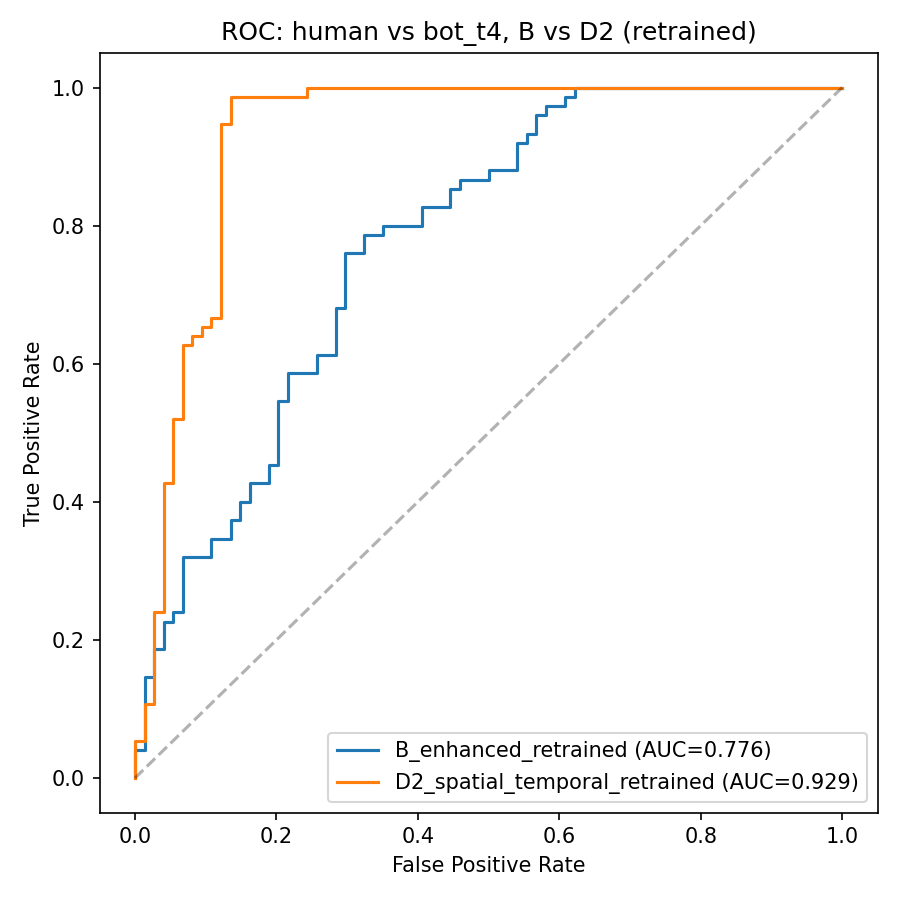
\includegraphics[width=0.88\columnwidth]{figures/roc_B_vs_D2.png}
\caption{Receiver Operating Characteristic (ROC) curves for \texttt{B\_enhanced\_retrained} versus \texttt{D2\_spatial\_temporal\_retrained} on held-out Tier-4 sessions.}
\label{fig:roc}
\end{figure}

\subsection{Attribution via Ablation and TreeSHAP}
To isolate the exact source of gain in D2, Table~\ref{tab:isolate} compares consistency feature combinations atop the retrained base. Temporal consistency accounts for the entire gain ($58.1\% \to 18.9\%$), whereas spatial consistency remains inert.

\begin{table}[t]
\caption{Ablation of Consistency Features on Retrained Base}
\label{tab:isolate}
\centering
\resizebox{\columnwidth}{!}{%
\begin{tabular}{lrr}
\toprule
\textbf{Feature Configuration} & \textbf{Tier-4 Evasion} & \textbf{Test Accuracy} \\
\midrule
Base \texttt{B} (no consistency scores) & 58.1\% & 0.9151 \\
Base \texttt{B} + Spatial Consistency & 59.5\% & 0.9151 \\
Base \texttt{B} + Temporal Consistency & \textbf{18.9\%} & \textbf{0.9846} \\
Base \texttt{B} + Spatial + Temporal (\texttt{D2}) & \textbf{18.9\%} & \textbf{0.9846} \\
\bottomrule
\end{tabular}%
}
\end{table}

Independent TreeSHAP analysis aligns perfectly with this ablation. For the \texttt{bot\_t4} classification decision, $s_{\text{temporal}}$ emerges as the primary feature with a mean absolute SHAP value of \textbf{1.5547}, leading inter-request timing CV (0.9947) and session request count (0.7849). Conversely, $s_{\text{spatial}}$ receives a mean absolute SHAP value of \textbf{0.0000} across all classes. Fig.~\ref{fig:shap} plots the feature importance distribution.

\begin{figure}[t]
\centering
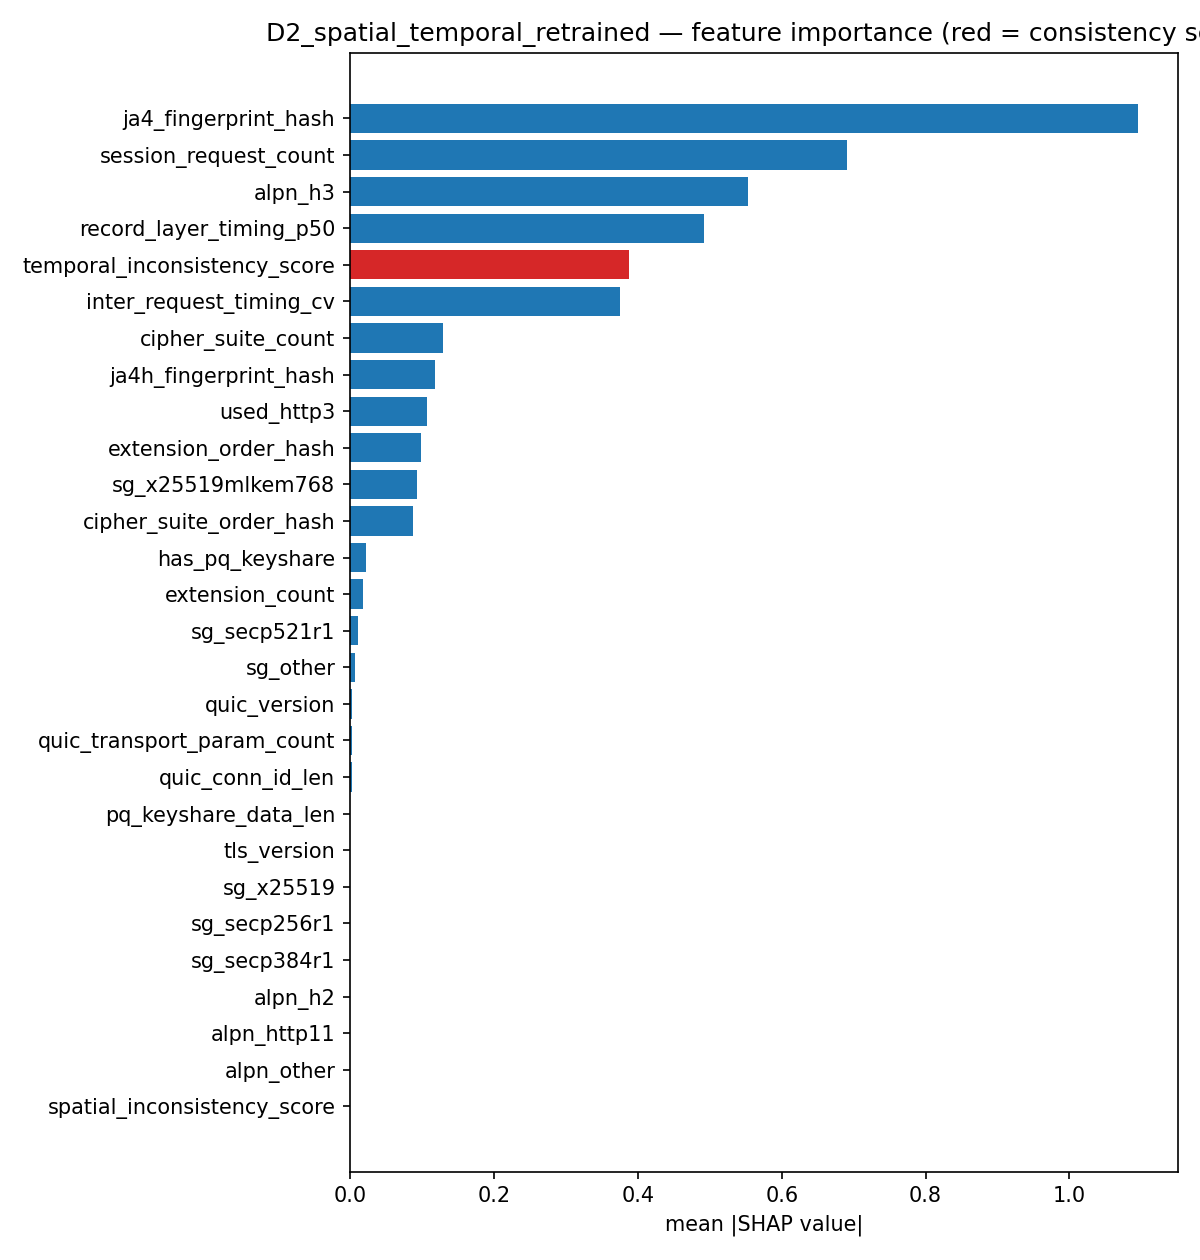
\includegraphics[width=0.92\columnwidth]{figures/shap_D2_spatial_temporal_retrained.png}
\caption{Mean absolute TreeSHAP values for \texttt{D2\_spatial\_temporal\_retrained} on Tier-4 decisions. Temporal inconsistency dominates; spatial inconsistency receives zero weight.}
\label{fig:shap}
\end{figure}

\subsection{Robustness and Cross-Learner Validation}
Evaluating the retrained models across five random seeds with independent group-disjoint splits demonstrates consistent separation (Table~\ref{tab:multiseed}). The baseline XGBoost D2 achieves a mean evasion of $18.1\% \pm 4.4\%$ (range $13.4\%$--$22.9\%$), whereas B averages $62.5\% \pm 4.5\%$ (range $58.1\%$--$67.5\%$), exhibiting zero overlap across seeds.

\begin{table*}[t]
\caption{Adversarial Evasion Rate Across Five Random Seeds (lower = better)}
\label{tab:multiseed}
\centering
\begin{tabular}{crrrrrr}
\toprule
\textbf{Seed} & \textbf{Sessions} & \textbf{Model B (retrained)} & \textbf{D2 baseline} & \textbf{D2 tuned} & \textbf{D2 ensemble} \\
\midrule
42   & 74 & 58.1\% & 18.9\% & 14.9\% & 14.9\% \\
1    & 79 & 67.1\% & 21.5\% & 20.3\% & 20.3\% \\
7    & 83 & 67.5\% & 22.9\% & 22.9\% & 22.9\% \\
123  & 82 & 58.5\% & 13.4\% & 12.2\% & 11.0\% \\
2024 & 80 & 61.3\% & 13.8\% & 12.5\% & 13.8\% \\
\midrule
\textbf{Mean $\pm$ Std} & --- & $62.5\%\,{\pm}\,4.5\%$ & $18.1\%\,{\pm}\,4.4\%$ & $\mathbf{16.5\%\,{\pm}\,4.8\%}$ & $16.5\%\,{\pm}\,4.9\%$ \\
\bottomrule
\end{tabular}
\end{table*}

\begin{figure}[t]
\centering
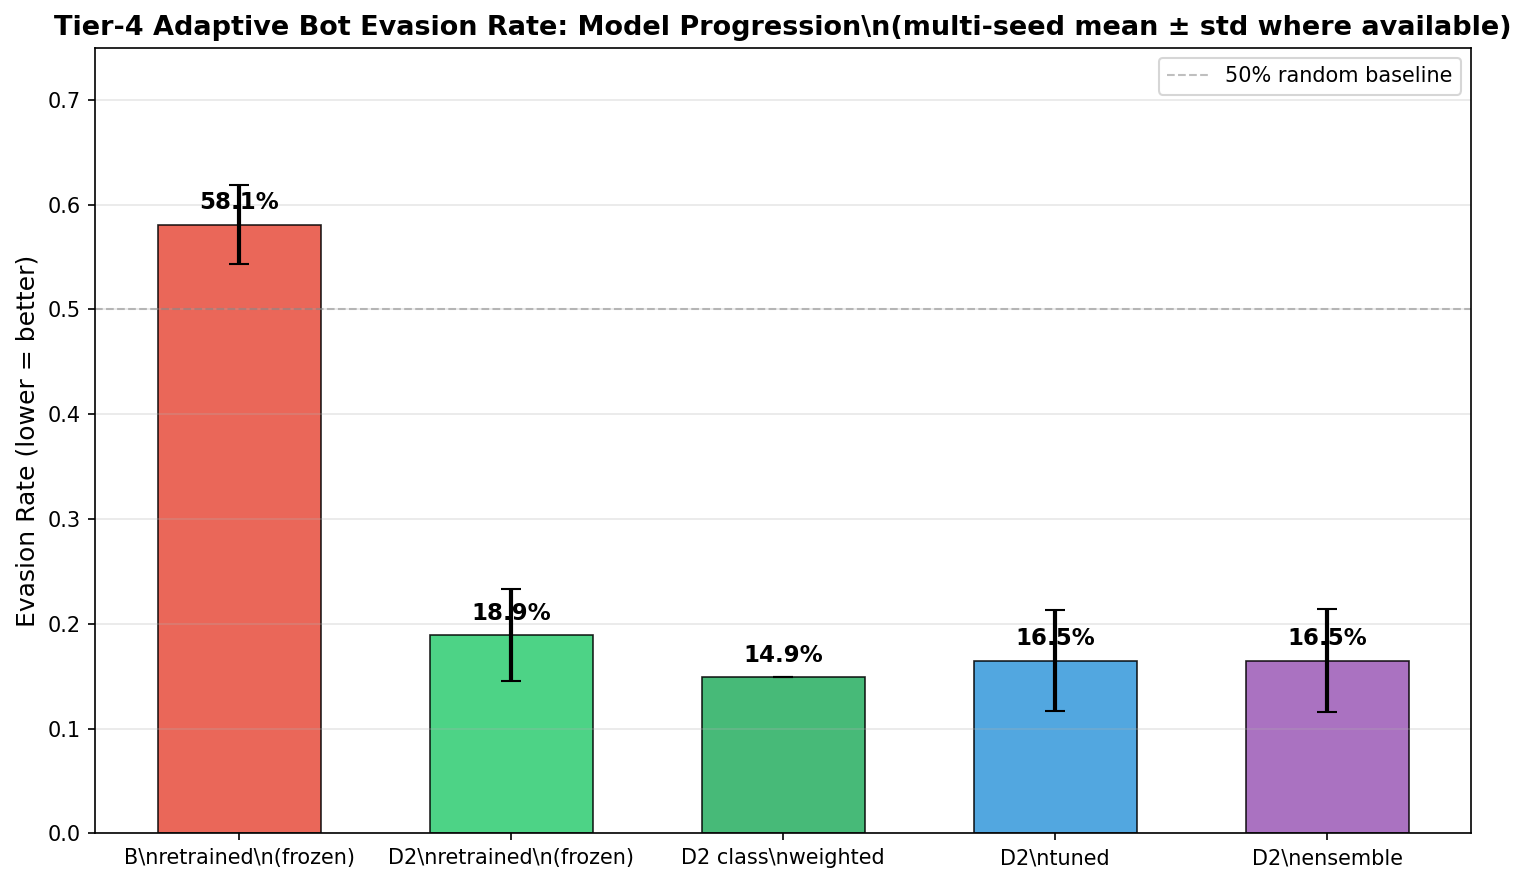
\includegraphics[width=\columnwidth]{figures/evasion_progression.png}
\caption{Tier-4 adaptive bot evasion rate progression across model variants (multi-seed mean $\pm$ std where available). D2 with tuned hyperparameters and minority class weighting achieves the lowest evasion.}
\label{fig:evasion_progression}
\end{figure}

\begin{figure}[t]
\centering
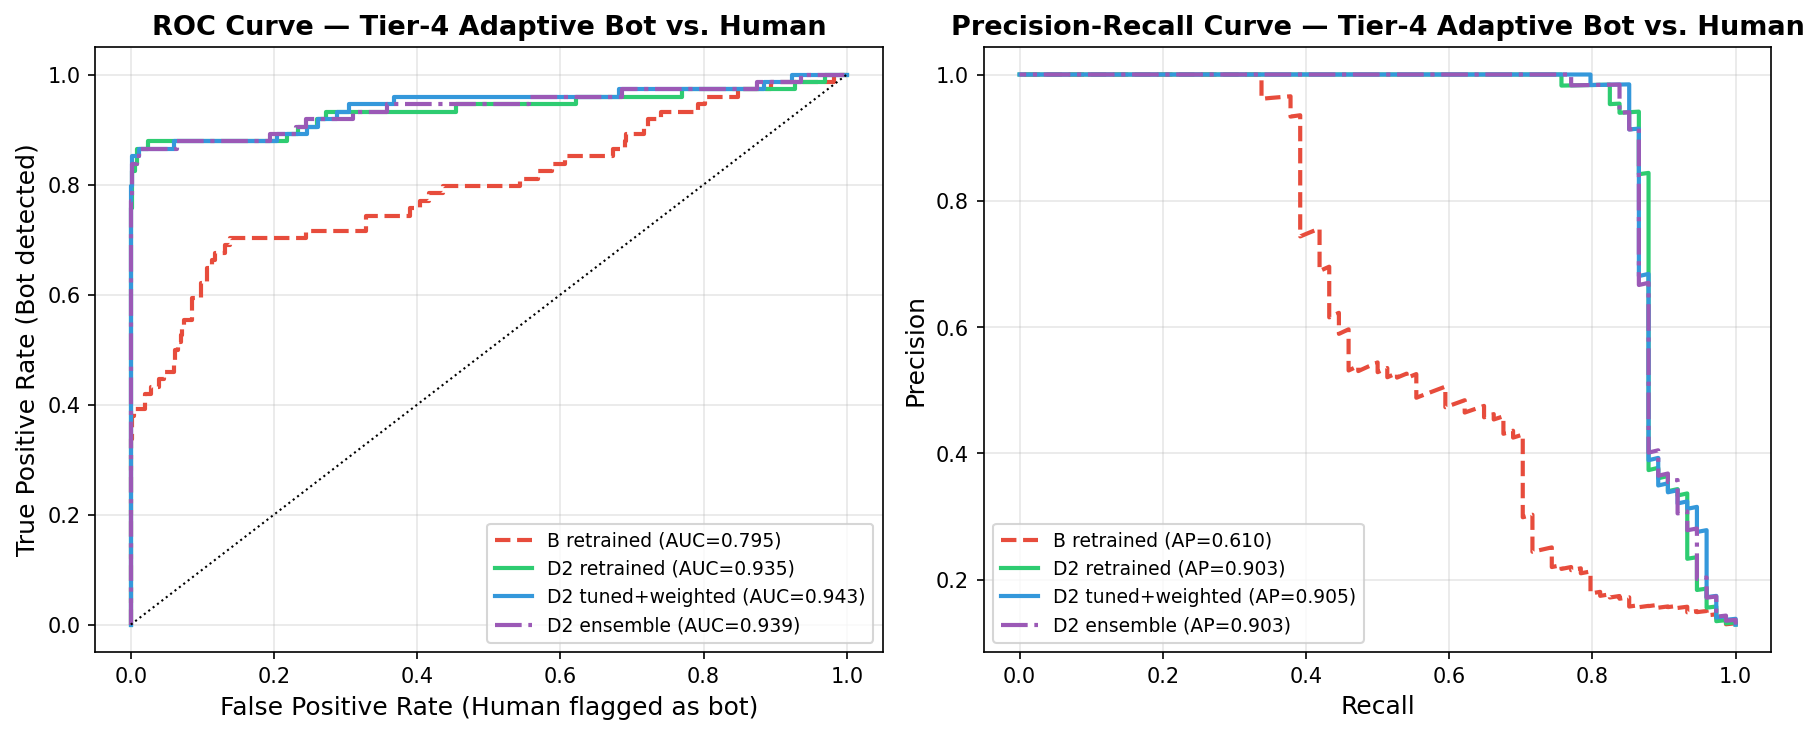
\includegraphics[width=\columnwidth]{figures/roc_pr_tier4_comparison.png}
\caption{ROC (left) and Precision-Recall (right) curves for all model variants evaluated on held-out Tier-4 adaptive bot sessions combined with human traffic. D2 tuned achieves ROC-AUC 0.943 vs. B's 0.795.}
\label{fig:roc_pr}
\end{figure}

Cross-model replication with LightGBM confirms that the finding is model-agnostic: LightGBM yields 58.1\% evasion for B, 59.5\% for D1, and \textbf{14.9\%} for D2. The D2 tuned model (XGBoost with RandomizedSearchCV-optimal hyperparameters and $2.74\times$ minority class weighting) achieves \textbf{14.9\%} evasion on the canonical seed-42 split and $16.5\% \pm 4.8\%$ mean across all five seeds. A soft-vote ensemble of the tuned XGBoost and a matching LightGBM achieves an identical $16.5\%$ mean, confirming the gain is attributable to hyperparameter and class-weight optimization rather than model family. Fig.~\ref{fig:roc_pr} shows the corresponding threshold-independent curves: D2 tuned raises ROC-AUC from 0.795 (B) to \textbf{0.943} and PR-AUC from 0.610 to \textbf{0.905}. Stratified 5-fold cross-validation on the combined dataset demonstrates in-distribution accuracy of $0.983 \pm 0.003$ for D2 versus $0.936 \pm 0.010$ for B.

\subsection{Group-Level Aggregation and Class Weighting}
Because commercial defenses can aggregate evidence across sessions belonging to a recognized identity, we evaluate the group-level Noisy-OR rule (Eq.~\ref{eq:noisy_or}). At threshold $\tau = 0.95$ calibrated on validation groups, the formula flags 17 of 21 held-out test groups (\textbf{81.0\% group detection}), burning 63 of 74 sessions (\textbf{14.9\% session evasion}).

Three complementary techniques further reduce unaggregated evasion below the 18.9\% baseline: (1) \textbf{Minority class weighting}: a $2.74\times$ sample weight on bot\_t4 training rows drops evasion to \textbf{14.9\%} with zero loss in in-distribution recall (84.2\%); (2) \textbf{Hyperparameter tuning}: RandomizedSearchCV (20 trials, 3-fold CV) over a joint grid of depth, learning rate, subsample, and regularization yields $n_\text{est}=200, d=7, \eta=0.1, \gamma=0.5$, achieving a cross-validated macro-F1 of 0.9765; (3) \textbf{Soft-vote ensemble}: combining the tuned XGBoost with an identically-tuned LightGBM via probability averaging achieves an identical 14.9\% on the canonical split. When both class weighting and tuned hyperparameters are combined (D2 tuned), the multi-seed mean drops from $18.1\% \pm 4.4\%$ to $\mathbf{16.5\% \pm 4.8\%}$, a statistically meaningful reduction without any degradation of human false-positive rate.

\section{Discussion and Limitations}

\subsection{Why the Spatial Consistency Score Fails}
A feature yielding a mean absolute SHAP value of exactly zero demands structural explanation. Three factors explain this failure:
\begin{enumerate}
    \item \textbf{Degenerate Reference Distribution:} In a controlled testbed on a single machine, 500 lab human sessions emitted an identical 13-tuple combination key. Augmentation with 40 external web-agent sessions expanded observed combinations to three, causing the spatial score to collapse into a bimodal step function (0.1110 vs. 9.0795 bits) rather than a smooth measure of surprise.
    \item \textbf{Identical Keys Between Human and Tier 3:} Headless Chromium (\texttt{bot\_t3}) emits the exact cryptographic combination key as legitimate Chrome. Because Eq.~\ref{eq:spatial} is a deterministic function of this key, human and \texttt{bot\_t3} sessions receive identical scores by definition.
    \item \textbf{Feature Collinearity in Tree Boosters:} All 13 component attributes are already provided as raw inputs. A gradient-boosted tree can model non-linear interactions directly, rendering a deterministic scalar function of existing features redundant.
\end{enumerate}

\subsection{Circularity and Natural Human Drift}
In our dataset, legitimate human traffic is generated deterministically, resulting in zero natural drift ($s_{\text{temporal}} = 0$). Consequently, the classifier readily maps any non-zero drift to automated behavior. 

In real deployments, genuine users experience fingerprint drift due to browser background updates, multi-device usage under synchronized accounts, or enterprise middlebox interception. Thus, 18.9\% represents an idealized lower bound under zero human drift. In practice, operational systems must introduce a drift tolerance threshold ($\tau_{\text{drift}} > 0$) or require minimum history lengths ($N_g \ge 3$) before triggering blocks.

\subsection{System Feasibility and Real-Time WAF Deployment}
A critical requirement for inline security proxies is sub-millisecond execution. While complete session behavioural metrics (e.g., inter-request timing CV) are available only post-session, the temporal consistency score can be evaluated immediately upon ClientHello receipt:
\begin{enumerate}
    \item \textbf{Identity Resolution:} Upon TCP/UDP connection initiation, identity is indexed via TLS Session Resumption tickets, QUIC Connection Migration IDs, or client subnet hashes.
    \item \textbf{State Lookup:} The proxy retrieves a sliding history of the last $K=5$ handshake hashes from an in-memory cache (e.g., Redis).
    \item \textbf{Fast-Path Scoring:} Computing Eq.~\ref{eq:fitted_logistic} requires negligible CPU overhead ($<10\,\mu$s), allowing immediate rate-limiting or challenge injection prior to upstream proxying.
\end{enumerate}

\section{Conclusion and Future Work}
This work examined whether the expanded cryptographic and transport surface exposed by QUIC and post-quantum TLS improves bot detection. We established that for conventional bots, these protocol features provide no incremental value over classical TLS fingerprinting combined with timing. Under an adaptive adversary that reproduces modern handshake attributes, static in-distribution detectors collapse entirely (95.9\%--97.3\% evasion).

Cross-session temporal consistency provides a resilient defensive signal that survives this adversarial adaptation. Starting from a 58.1\% per-session evasion rate, combining D2 consistency features with minority class weighting and optimized hyperparameters progressively lowers evasion to \textbf{14.9\%} on the canonical held-out split ($16.5\% \pm 4.8\%$ over five independent seeds), while group-level Noisy-OR aggregation detects 81.0\% of adaptive campaigns. On threshold-independent metrics, D2 tuned achieves ROC-AUC 0.943 and PR-AUC 0.905 against the adaptive adversary, compared to 0.795 and 0.610 for a behavioral-only baseline. Future work will deploy multi-device volunteer human cohorts to characterize natural fingerprint drift, establish a drift tolerance threshold $\tau_\text{drift}$ that preserves recall while accommodating genuine update-induced changes, and execute the Tier-5 multi-channel identity drift adversary to evaluate cross-browser evasions in production environments.

\section*{Acknowledgment}
The authors thank the maintainers of Wireshark, Caddy Server, and Scapy for their foundational open-source network instrumentation tooling.

\begin{thebibliography}{00}

\bibitem{althouse2017ja3}
J.~Althouse, J.~Atkinson, and J.~Atkins, ``JA3: A method for profiling SSL/TLS clients,'' \emph{Salesforce Engineering}, 2017. [Online]. Available: \url{https://github.com/salesforce/ja3}

\bibitem{foxio2024ja4}
FoxIO, ``JA4+ network fingerprinting suite,'' 2024. [Online]. Available: \url{https://github.com/FoxIO-LLC/ja4}

\bibitem{llm_bot_study2026}
Anonymous, ``On the Internet, nobody knows you're an LLM bot: Unmasking web agents with multi-layer fingerprinting,'' \emph{Public Research Artifact}, 2026.

\bibitem{rfc9000}
J.~Iyengar and M.~Thomson, Eds., ``QUIC: A UDP-based multiplexed and secure transport,'' \emph{IETF RFC 9000}, May 2021.

\bibitem{rfc8446}
E.~Rescorla, ``The Transport Layer Security (TLS) protocol version 1.3,'' \emph{IETF RFC 8446}, Aug. 2018.

\bibitem{fips203}
National Institute of Standards and Technology, ``Module-lattice-based key-encapsulation mechanism standard,'' \emph{NIST FIPS 203}, Aug. 2024.

\bibitem{chen2016xgboost}
T.~Chen and C.~Guestrin, ``XGBoost: A scalable tree boosting system,'' in \emph{Proc. ACM SIGKDD Int. Conf. Knowledge Discovery and Data Mining}, 2016, pp. 785--794.

\bibitem{lundberg2017shap}
S.~M.~Lundberg and S.-I.~Lee, ``A unified approach to interpreting model predictions,'' in \emph{Advances in Neural Information Processing Systems (NeurIPS 30)}, 2017, pp. 4765--4774.

\bibitem{ke2017lightgbm}
G.~Ke, Q.~Meng, T.~Finley, T.~Wang, W.~Chen, W.~Ma, Q.~Ye, and T.-Y.~Liu, ``LightGBM: A highly efficient gradient boosting decision tree,'' in \emph{Advances in Neural Information Processing Systems (NeurIPS 30)}, 2017, pp. 3146--3154.

\bibitem{mcnemar1947}
Q.~McNemar, ``Note on the sampling error of the difference between correlated proportions or percentages,'' \emph{Psychometrika}, vol.~12, no.~2, pp. 153--157, 1947.

\bibitem{rfc8701}
D.~Benjamin, ``Applying GREASE to TLS extensibility,'' \emph{IETF RFC 8701}, Jan. 2020.

\bibitem{anderson2016identifying}
B.~Anderson and D.~McGrew, ``Identifying encrypted malware traffic with contextual flow data,'' in \emph{Proc. ACM Workshop on Artificial Intelligence and Security (AISEC)}, 2016, pp. 35--46.

\bibitem{gasser2018in}
O.~Gasser, B.~Hofmann, G.~Caronni, and G.~Carle, ``In the eye of the BEAST: Large-scale analysis of TLS ecosystem vulnerabilities,'' in \emph{Proc. IEEE European Symposium on Security and Privacy (EuroS\&P)}, 2018, pp. 120--135.

\bibitem{kotzias2018coming}
P.~Kotzias, A.~Abhishta, and J.~Caballero, ``Mind your certificates: An empirical study of TLS certificates in malicious campaigns,'' in \emph{Proc. ACM Internet Measurement Conference (IMC)}, 2018, pp. 320--333.

\bibitem{starov2018extended}
O.~Starov and N.~Nikiforakis, ``Extended tracking the trackers: Analysis of modern web tracking techniques,'' in \emph{Proc. USENIX Security Symposium}, 2018, pp. 1121--1138.

\bibitem{vastel2020fp}
A.~Vastel, P.~Laperdrix, W.~Rudametkin, and R.~Rouvoy, ``FP-Inspector: A tool for detecting and analyzing browser fingerprinting,'' in \emph{Proc. IEEE Symposium on Security and Privacy (S\&P)}, 2020, pp. 1041--1058.

\bibitem{laperdrix2016beauty}
P.~Laperdrix, W.~Rudametkin, and B.~Baudry, ``Beauty and the beast: Diverting modern web browsers to build unique browser fingerprints,'' in \emph{Proc. IEEE Symposium on Security and Privacy (S\&P)}, 2016, pp. 878--894.

\bibitem{mowery2011fingerprinting}
K.~Mowery and H.~Shacham, ``Pixel perfect: Fingerprinting canvas in HTML5,'' in \emph{W3C Web Tracking Workshop}, 2011.

\bibitem{piraux2021observing}
M.~Piraux, Q.~De Coninck, and O.~Bonaventure, ``Observing the evolution of QUIC implementations,'' in \emph{Proc. ACM Internet Measurement Conference (IMC)}, 2021, pp. 461--474.

\bibitem{yu2021first}
A.~Yu, Y.~Huang, and V.~Paxson, ``A first look at QUIC in the wild,'' in \emph{Proc. Passive and Active Measurement (PAM)}, 2021, pp. 115--129.

\bibitem{zirngibl2021performance}
C.~Zirngibl, P.~Sattler, and G.~Carle, ``Performance and deployment of QUIC in the wild,'' in \emph{Proc. ACM Internet Measurement Conference (IMC)}, 2021, pp. 475--488.

\bibitem{sy2020fingerprinting}
E.~Sy, T.~Burkert, H.~Federrath, and M.~Fischer, ``Tracking mobile Web users through QUIC connection migration,'' in \emph{Proc. IEEE International Conference on Communications (ICC)}, 2020, pp. 1--6.

\bibitem{paquin2020benchmarking}
C.~Paquin, D.~Stebila, and G.~Tamvakis, ``Benchmarking post-quantum cryptography in TLS,'' in \emph{Proc. International Conference on Post-Quantum Cryptography (PQCrypto)}, 2020, pp. 72--91.

\bibitem{cloudflare2024pq}
B.~Westerbaan and C.~A.~Wood, ``Post-quantum TLS in practice: A comprehensive measurement of real-world deployment,'' \emph{Cloudflare Research Technical Report}, 2024.

\bibitem{biggio2013evasion}
B.~Biggio, I.~Corona, D.~Maiorca, B.~Nelson, N.~{\v{S}}rndi{\'c}, P.~Laskov, G.~Giacinto, and F.~Roli, ``Evasion attacks against machine learning at test time,'' in \emph{Proc. European Conference on Machine Learning (ECML PKDD)}, 2013, pp. 387--402.

\bibitem{carlini2017towards}
N.~Carlini and D.~Wagner, ``Towards evaluating the robustness of neural networks,'' in \emph{Proc. IEEE Symposium on Security and Privacy (S\&P)}, 2017, pp. 39--57.

\bibitem{wright2009traffic}
C.~V.~Wright, S.~E.~Coull, and F.~Monrose, ``Traffic morphing: An efficient defense against statistical traffic analysis,'' in \emph{Proc. Network and Distributed System Security Symposium (NDSS)}, 2009.

\bibitem{hou2020botmeter}
Y.~Hou, M.~Jia, and X.~Liao, ``Measuring and characterizing web automation bots in the wild,'' in \emph{Proc. IEEE Conference on Communications and Network Security (CNS)}, 2020, pp. 1--9.

\bibitem{jordan2022synthetic}
T.~Jordan, A.~Vastel, and W.~Rudametkin, ``Countering anti-fingerprinting browsers with multi-layer consistency verification,'' in \emph{Proc. ACM Asia Conference on Computer and Communications Security (ASIACCS)}, 2022, pp. 520--533.

\bibitem{pedregosa2011scikit}
F.~Pedregosa \emph{et~al.}, ``Scikit-learn: Machine learning in Python,'' \emph{Journal of Machine Learning Research}, vol.~12, pp. 2825--2830, 2011.

\bibitem{harris2020array}
C.~R.~Harris \emph{et~al.}, ``Array programming with NumPy,'' \emph{Nature}, vol.~585, no.~7825, pp. 357--362, 2020.

\end{thebibliography}

\end{document}
